% Unit 060 terjemahan Bahasa Indonesia dari chapter4.tex baris 2002--2115.
% Sumber: Methods of Algebra, Volume 2, commit
% 9a5803ff77dd3257484cb177f851a73770a59dd3 (CC BY 4.0).
% stable-unit-id: o014.aljabr2.chapter4.rlim-homotopy-limit
% Cakupan: Bagian 4.10 lengkap; berhenti sebelum Bagian 4.11 pada baris 2116.

% segment-id: o014.li2.chapter4.rlim-homotopy-limit.h001
\section{Contoh: \texorpdfstring{$\mathrm{R}\lim$}{Rlim} sebagai Limit Homotopi}\label{sec:Rlim}
\hypertarget{o014.aljabr2.chapter4.rlim-homotopy-limit}{ }

% segment-id: o014.li2.chapter4.rlim-homotopy-limit.p001
Bagian ini melanjutkan pembahasan \S\ref{sec:lim1}. Misalkan $\mathcal{A}$
suatu kategori abelian.

% segment-id: o014.li2.chapter4.rlim-homotopy-limit.l001
\begin{lema}\label{prop:D-countable-product}
	Misalkan $\mathcal{A}$ mempunyai produk terhitung eksak (atau koproduk
	terhitung eksak), lihat Konvensi~\ref{con:exact-product}. Maka setiap funktor
	dalam rangkaian
	$\cate{C}(\mathcal{A})\to\cate{K}(\mathcal{A})\to\cate{D}(\mathcal{A})$
	mempertahankan produk terhitung (atau koproduk terhitung). Dalam hal ini
	terdapat isomorfisme kanonik
	$\Hm^n(\prod_kX_k)\rightiso\prod_k\Hm^n(X_k)$ (atau
	$\Hm^n(\bigoplus_kX_k)\rightiso\bigoplus_k\Hm^n(X_k)$).
\end{lema}
% segment-id: o014.li2.chapter4.rlim-homotopy-limit.pf001
\begin{bukti}
	Cukup membuktikan kasus produk. Keeksakan produk terhitung langsung memberikan
	$\Hm^n(\prod_kX_k)\rightiso\prod_k\Hm^n(X_k)$.

	Untuk setiap kompleks $Y$, dari definisi terlihat bahwa
	$\Hom^\bullet(Y,\prod_kX_k)$ isomorfik dengan produk
	$\Hom^\bullet(Y,X_k)$ yang dibentuk derajat demi derajat dalam
	$\cate{C}(\cate{Ab})$. Terapkan keeksakan produk terhitung saat mengambil
	$\Hm^0$ untuk memperoleh isomorfisme kanonik
	$\Hom_{\cate{K}(\mathcal{A})}(Y,\prod_kX_k)\simeq
	\prod_k\Hom_{\cate{K}(\mathcal{A})}(Y,X_k)$. Jadi
	$\cate{C}(\mathcal{A})\to\cate{K}(\mathcal{A})$ mempertahankan $\prod_k$.

	Sekarang kita buktikan bahwa
	$\cate{K}(\mathcal{A})\to\cate{D}(\mathcal{A})$ mempertahankan $\prod_k$;
	funktor lokalisasi $Q$ tidak dituliskan. Misalkan diberikan keluarga morfisme
	$f_k:Y\to X_k$ dalam $\cate{D}(\mathcal{A})$. Kita hendak membuktikan bahwa
	terdapat tepat satu
	$f\in\Hom_{\cate{D}(\mathcal{A})}(Y,\prod_kX_k)$ yang memenuhi
	$p_hf=f_h$ untuk setiap $h$, dengan
	$p_h:\prod_kX_k\to X_h$ proyeksi kanonik dalam $\cate{K}(\mathcal{A})$.
	Kita boleh mengandaikan bahwa $f_k$ berasal dari diagram dalam
	$\cate{K}(\mathcal{A})$
	\begin{equation}\label{eqn:D-countable-product-aux0}
		Y \xrightarrow{b_k} Z_k \xleftarrow{s_k} X_k, \quad s_k:\; \text{kuasi-isomorfisme}.
	\end{equation}
	Morfisme
	$s:=\prod_ks_k:\prod_kX_k\to\prod_kZ_k$ tetap merupakan kuasi-isomorfisme.
	Diagram
	\[ Y \xrightarrow{b := (b_k)_k} \prod_k Z_k \xleftarrow{s} \prod_k X_k \]
	menentukan $f\in\Hom_{\cate{D}(\mathcal{A})}(Y,\prod_kX_k)$. Perhatikan
	bahwa $f$ tidak bergantung pada pilihan dalam
	\eqref{eqn:D-countable-product-aux0}, melainkan hanya pada $(f_k)_k$.
	Komutativitas diagram berikut menyiratkan $p_hf=f_h$ untuk setiap $h$:
% segment-id: o014.li2.chapter4.rlim-homotopy-limit.g001
	\[\begin{tikzcd}
		& Z_h & X_h \arrow[l, "s_h"'] \\
		Y \arrow[r, "b"'] \arrow[ru, "b_h"] & \prod_k Z_k \arrow[u] & \prod_k X_k \arrow[l, "s"] \arrow[u, "p_h"'] .
	\end{tikzcd} \]

	Jika $g\in\Hom_{\cate{D}(\mathcal{A})}(Y,\prod_kX_k)$ juga memenuhi
	$p_hg=f_h$ untuk setiap $h$, terdapat diagram komutatif dalam
	$\cate{K}(\mathcal{A})$
% segment-id: o014.li2.chapter4.rlim-homotopy-limit.g002
	\[\begin{tikzcd}
		& M_h & X_h \arrow[l, "t_h"'] \\
		Y \arrow[r, "c"] \arrow[ru, "c_h"] \arrow[rd, "{(c_k)_k}"'] & M \arrow[u, "r_h"'] \arrow[d, "(r_k)_k"] & \prod_k X_k \arrow[l, "t"'] \arrow[u, "p_h"'] \arrow[ld, "u"] \\
		& \prod_k M_k &
	\end{tikzcd} \quad \begin{array}{l}
		h \in \Z, \\
		t, t_h:\;\text{kuasi-isomorfisme}, \\
		u := (r_k)_k t = \prod_k t_k ,
	\end{array}\]
	sedemikian sehingga baris kedua menentukan $g$, sedangkan bagian
	$\begin{tikzpicture}[xscale=0.3, yscale=0.3, baseline=(O)]
		\coordinate (O) at (0, -0.8);
		\draw[->] (0,-1) -- (1, 0) -- (2, 0);
	\end{tikzpicture}$
	menentukan $f_h$. Konstruksi bagian perseginya menggunakan versi kondisi
	(S3) dalam Definisi~\ref{def:multiplicative-family} bagi sistem
	multiplikatif kanan, sedangkan komutativitas bagian bawah langsung.

	Keeksakan $\prod_k$ menunjukkan bahwa $u$ merupakan kuasi-isomorfisme.
	Akibatnya, $g$ juga ditentukan oleh bagian
	$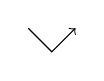
\begin{tikzpicture}[xscale=0.3, yscale=0.3, baseline=(O)]
		\coordinate (O) at (0, -0.8);
		\draw[->] (0,0) -- (1, -1) -- (2, 0);
	\end{tikzpicture}$
	dari diagram. Namun, $Y\xrightarrow{c_k}M_k\xleftarrow{t_k}X_k$
	menentukan $f_k$. Dibandingkan dengan konstruksi $f$ di atas, diperoleh
	$f=g$. Terbukti.
\end{bukti}

% segment-id: o014.li2.chapter4.rlim-homotopy-limit.r001
\begin{catatan}
	Jika himpunan indeks produk (atau koproduk) diganti dengan sembarang himpunan
	kecil $I$, pernyataan yang bersesuaian tetap berlaku.
\end{catatan}

% segment-id: o014.li2.chapter4.rlim-homotopy-limit.p002
Misalkan $\mathcal{D}$ suatu kategori-$\cate{Ab}$. Tinjau kategori
$\cate{InvSys}(\mathcal{D}):=\mathcal{D}^{\Z_{\geq0}^{\opp}}$ dari
\eqref{eqn:InvSys}. Objeknya adalah data $X=(X_k,f_k)_{k\geq0}$, dengan
$X_k\in\Obj(\mathcal{D})$ dan
$f_k\in\Hom_{\mathcal{D}}(X_{k+1},X_k)$. Jika $\mathcal{D}$ mempunyai produk
terhitung, definisikan morfisme kanonik seperti dalam
Definisi~\ref{def:Delta-diff}:
	\[ \Delta_X := T_X - \identity: \prod_k X_k \to \prod_k X_k. \]
\index[sym1]{InvSys}
\index[sym1]{DirSys@$\cate{DirSys}$}

% segment-id: o014.li2.chapter4.rlim-homotopy-limit.p003
Secara dual, objek kategori
$\cate{DirSys}(\mathcal{D}):=\mathcal{D}^{\Z_{\geq0}}$ adalah data
$X=(X_k,g_k)_{k\geq0}$\footnote{Data ini juga disebut sistem langsung dalam
$\mathcal{D}$.}, dengan $X_k\in\Obj(\mathcal{D})$ dan
$g_k\in\Hom_{\mathcal{D}}(X_k,X_{k+1})$. Dengan cara yang sama, definisikan
$\nabla_X:=T_X-\identity:\bigoplus_kX_k\to\bigoplus_kX_k$, dengan asumsi
$\mathcal{D}$ mempunyai koproduk terhitung; $T_X$ tetap merupakan morfisme
pergeseran yang serupa.

% segment-id: o014.li2.chapter4.rlim-homotopy-limit.p004
Jika $\Ker(\Delta_X)$ atau $\Coker(\nabla_X)$ ada, terdapat isomorfisme
kanonik
\begin{align*}
	X \in \Obj\left( \cate{InvSys}(\mathcal{D}) \right) & \implies \varprojlim_k X_k \simeq \Ker(\Delta_X), \\
	X \in \Obj\left( \cate{DirSys}(\mathcal{D}) \right) & \implies \varinjlim_k X_k \simeq \Coker(\nabla_X).
\end{align*}
Harapan naifnya ialah menerapkan ini pada $\mathcal{D}=\cate{D}(\mathcal{A})$.
Kategori turunan jarang merupakan kategori abelian. Meskipun demikian,
Catatan~\ref{rem:homotopy-kernel-cokernel} menunjukkan bahwa kerucut pemetaan
dapat berperan sebagai versi homotopis dari kernel dan kokernel; konstruksi yang
secara kasar bersesuaian dalam kategori bertriangulasi adalah segitiga
terbedakan.

% segment-id: o014.li2.chapter4.rlim-homotopy-limit.d001
\begin{definisi}[M.\ Bökstedt, A.\ Neeman {\cite{BN93}}]\label{def:holim}
	\index{limit homotopi, kolimit homotopi}
	\index[sym1]{holim@$\holim$, $\hocolim$}
	Misalkan $\mathcal{D}$ kategori bertriangulasi.
	\begin{itemize}
		\item Jika $\mathcal{D}$ mempunyai produk terhitung, suatu \emph{limit
		homotopi} (atau $\varprojlim$ homotopi) dari objek
		$X\in\Obj(\cate{InvSys}(\mathcal{D}))$ berarti segitiga terbedakan
		\[ \holim(X) \to \prod_k X_k \xrightarrow{\Delta_X} \prod_k X_k \xrightarrow{+1} . \]
		\item Jika $\mathcal{D}$ mempunyai koproduk terhitung, suatu
		\emph{kolimit homotopi} (atau $\varinjlim$ homotopi) dari objek
		$X\in\Obj(\cate{DirSys}(\mathcal{D}))$ berarti segitiga terbedakan
		\[ \bigoplus_k X_k \xrightarrow{\nabla_X} \bigoplus_k X_k \to \hocolim(X) \xrightarrow{+1} . \]
	\end{itemize}
\end{definisi}

% segment-id: o014.li2.chapter4.rlim-homotopy-limit.p005
Segitiga-segitiga terbedakan yang terlibat dalam definisi ini saling isomorfik
(Korolari~\ref{prop:Cone-uniqueness}), tetapi isomorfismenya tidak kanonik.

% segment-id: o014.li2.chapter4.rlim-homotopy-limit.p006
Kembali ke kompleks. Perhatikan bahwa
$\cate{InvSys}(\cate{C}(\mathcal{A}))=
\cate{C}(\cate{InvSys}(\mathcal{A}))$; objek kedua kategori tersebut sama-sama
merupakan diagram komutatif
% segment-id: o014.li2.chapter4.rlim-homotopy-limit.g003
\[\begin{tikzcd}
	& \vdots \arrow[d, "{f_1^n}"'] & \vdots \arrow[d, "{f_1^{n+1}}"] & \\
	\cdots \arrow[r] & X_1^n \arrow[r, "{d_{X_1}^n}"] \arrow[d, "{f_0^n}"'] & X_1^{n+1} \arrow[d, "{f_0^{n+1}}"] \arrow[r] & \cdots \\
	\cdots \arrow[r] & X_0^n \arrow[r, "{d_{X_0}^n}"] & X_0^{n+1} \arrow[r] & \cdots
\end{tikzcd} \quad \text{dengan setiap baris merupakan kompleks}. \]
Morfisme di kedua kategori juga merupakan diagram komutatif dua tingkat yang
sama. Karena itu, dalam $\mathcal{D}:=\cate{D}(\mathcal{A})$ kita dapat
membandingkan $\holim(X)$ dan funktor turunan kanan
$\mathrm{R}\lim(X)$ dari $\varprojlim$, jika keduanya ada.

% segment-id: o014.li2.chapter4.rlim-homotopy-limit.p007
Perhatikan pula bahwa kohomologi $\Hm^m$ dari objek
$X\in\cate{C}(\cate{InvSys}(\mathcal{A}))$ adalah
$(\Hm^m(X_k),\Hm^m(f_k))_{k\geq0}$. Jadi $X\to Y$ merupakan
kuasi-isomorfisme jika dan hanya jika setiap $X_k\to Y_k$ merupakan
kuasi-isomorfisme dalam $\cate{C}(\mathcal{A})$.

% segment-id: o014.li2.chapter4.rlim-homotopy-limit.t001
\begin{teorema}\label{prop:Rlim-as-holim}
	Misalkan $\mathcal{A}$ kategori abelian dengan produk terhitung yang eksak
	dan cukup banyak objek injektif.
	\begin{enumerate}[(i)]
		\item Funktor turunan kanan dari funktor eksak kiri
		$\varprojlim:\cate{InvSys}(\mathcal{A})\to\mathcal{A}$ ada dan dituliskan
		\[ \mathrm{R}\lim :  \cate{D}^+\left(\cate{InvSys}(\mathcal{A})\right) \to \cate{D}^+(\mathcal{A}) . \]
		\item Untuk setiap objek $X=(X_k,f_k)_{k\geq0}$ dari
		$\cate{C}^+(\cate{InvSys}(\mathcal{A}))$, terdapat segitiga terbedakan
		dalam $\cate{D}(\mathcal{A})$
		\[ \mathrm{R}\lim(X) \to \prod_k X_k \xrightarrow{\Delta_X} \prod_k X_k \xrightarrow{+1}. \]
		Secara khusus, $\mathrm{R}\lim(X)\simeq\holim(X)$.
		\item Dimensi $\mathrm{R}\lim$ dalam pengertian
		Definisi--Proposisi~\ref{def:dim-functor} paling besar $1$.
	\end{enumerate}
\end{teorema}
% segment-id: o014.li2.chapter4.rlim-homotopy-limit.pf002
\begin{bukti}
	Karena $\cate{InvSys}(\mathcal{A})$ mempunyai cukup banyak objek injektif,
	(i) berlaku. Lebih tepatnya, ambil kategori $\mathcal{R}$ dari
	Lema~\ref{prop:lim1-prep} dan terapkan
	Teorema~\ref{prop:resolution-existence} pada
	$\cate{InvSys}(\mathcal{A})$ dan $\mathcal{R}$. Untuk setiap
	$X=(X_k,f_k)_{k\geq0}$ dalam
	$\cate{C}^+(\cate{InvSys}(\mathcal{A}))$, terdapat kuasi-isomorfisme
	$X\to Y$ dengan $Y\in\Obj(\cate{C}^+(\mathcal{R}))$. Maka
	$\mathrm{R}\lim(X)=\varprojlim Y$. Definisi $\mathcal{R}$ menjamin bahwa
	$\Delta_Y$ surjektif derajat demi derajat, sehingga terdapat barisan eksak
	pendek dalam $\cate{C}^+(\mathcal{A})$
	\[ 0 \to \varprojlim Y \to \prod_{k \geq 0} Y_k \xrightarrow{\Delta_Y} \prod_{k \geq 0} Y_k \to 0. \]
	Selanjutnya, setiap $X_k\to Y_k$ merupakan kuasi-isomorfisme, sehingga
	$\prod_{k\geq0}X_k\to\prod_{k\geq0}Y_k$ juga merupakan kuasi-isomorfisme.
	Ini memberikan segitiga terbedakan pada (ii):
	\[ \mathrm{R}\lim(X) \to \prod_{k \geq 0} X_k \xrightarrow{\Delta_X} \prod_{k \geq 0} X_k \xrightarrow{+1} . \]

	Untuk (iii), jika $X\in\Obj(\cate{InvSys}(\mathcal{A}))$, maka $\Delta_X$
	merupakan morfisme dalam $\cate{InvSys}(\mathcal{A})$, dan
	$\holim(X)\simeq\Cone(\Delta_X)[-1]$ berada dalam
	$\Obj(\cate{D}^{[0,1]}(\mathcal{A}))$. Ini juga merupakan pernyataan ulang
	Teorema~\ref{prop:lim1}.
\end{bukti}

% segment-id: o014.li2.chapter4.rlim-homotopy-limit.p008
Terdapat versi dual Teorema~\ref{prop:Rlim-as-holim} untuk
$\varinjlim:\cate{DirSys}(\mathcal{A})\to\mathcal{A}$; perinciannya tidak
diulangi.

% segment-id: o014.li2.chapter4.rlim-homotopy-limit.p009
Contoh~\ref{eg:Rlim-unbounded} akan menunjukkan cara memperoleh
$\mathrm{R}\lim$ pada kategori turunan tak terbatas sedemikian sehingga
Teorema~\ref{prop:Rlim-as-holim} (ii) tetap berlaku.
